
ILCS is a scalable framework for running iterative local searches on HPC platforms.
%
Providing a serial CPU or single-GPU code, ILCS then executes this code in parallel between compute nodes (MPI) and within them (OpenMP and multi-GPU).
%

To evaluate the effectiveness of ideas behind DiffTrace, we have manually injected MPI-level and OMP-level bugs to the Traveling Salesman Problem (TSP) implementation on ILCS framework (Listing~\ref{lst:ilcs}).
%
The injected bugs are tend to simulate real HPC bugs such as deadlocks.
%
Also bugs are close to common mistakes that HPC developers usually make during developing HPC codes.
%
In addition, there exist ``hidden'' faults that does not alarm anything during execution such as violation of critical sections or semantic-based bugs. 
%

\begin{frame}{}
  \lstset{language=C}
 \begin{lstlisting}[caption={ILCS Overview},label={lst:ilcs}]
main(argc, argv) {
 ... // initialization
 MPI_Init();
 MPI_Comm_size();
 MPI_Comm_rank(my_rank);
 ... // Obtain number of local CPUs and GPUs
 MPI_Reduce(lCPUs, gCPUs, MPI_SUM); // Total # of CPUs
 MPI_Reduce(lGPUs, gGPUs, MPI_SUM); // Total # of GPUs
 champSize = CPU_Init();
 ... // Memory allocation for storing local and global champions w.r.t. champSize
 MPI_Barrier();
 <@\textcolor{blue} {\#pragma omp parallel num\_threads(lCPUs+1)}@>
 {rank = omp_get_thread_num();
  if (rank != 0) { // worker threads
   while (cont) {
    ... // calculate seed
    local_result = CPU_Exec();
    if (local_result < champ[rank]) { // update local champion
     <@\textcolor{blue}{\#pragma omp critical}@>
     memcpy(champ[rank], local_result);}}
  } else { //master thread
   do {
    ...
    MPI_AllReduce(); //broadcast the global champion 
	  ...
    MPI_AllReduce(); //broadcast the global champion P_id
    ...
    if (my_rank == global_champion_P_id) {
     <@\textcolor{blue}{\#pragma omp critical}@>
     memcpy(bcast_buffer, champ[rank]);
    }
    MPI_Bcast(bcast_buffer); // broadcast the local champion to all nodes
   } while (no_change_threshold);
   cont = 0; // signal worker threads to terminate
  }}
 if (my_rank == 0) {CPU_Output(champ);}
 MPI_Finalize();}

/* User code for TSP problem */
CPU_Init() {/* Read coordinates, calculate distances, initialize champion structure, return structure size */}
CPU_Exec() {/* Find local champions (TSP tours) */}
CPU_Output() {/* Output champion */}
\end{lstlisting}
\end{frame}


The injected bugs are planted in a way that might get triggered in only one or more threads (master and worker threads, one thread, every other thread, all threads except one, all threads). 
%
Generally, the goal is to see how effective DiffTrace can analyze and diff traces, and how close it can get to the fault root cause or its manifestation. 

%
We have collected ParLOT (main image) traces from the execution of ILCS-TSP with 8 MPI processes and 4 OpenMP threads on each process. \hl{PSC Config will be added}. Note that the GPU-related activities of ILCS are out of the scope of this paper, and we have not touched them in our experiments.
Here, after a general explanation of ILCS behavior, we explain the injected bugs and the observations from DiffTrace.%


\subsection{ILCS-TSP workflow}

\hl{2-3 sentences about how ILCS finds local champions in TSP problem}

There are two types of threads in ILCS: a \textit{master} thread per node (MPI process) and a set of \textit{worker} threads per compute node (OpenMP threads).
%
Master threads of compute nodes are in charge of handling local working threads and communicating with master threads on other nodes.
%
For each detected CPU core, the master thread forks worker OpenMP threads.
%
Each worker thread continually calls
\texttt{CPU\_Exec()} to evaluate a range of seeds and record the results (lines 14-20).
%
Once the worker threads are running, the master thread's primary job is to scan the results of the workers to find the best solution computed so far (i.e., the local champion). This information is then globally reduced to determine the current system-wide champion (lines 22-32).
%
Since scanning the entire seed range in a reasonable amount of time is not feasible, ILCS terminates the search when the quality has not improved over a certain period (lines 33-34).

\subsection{OpenMP Bug: Unprotected Memory Access}


\begin{table*}[]
\centering
\caption{Ranking Table - OMP-Bug: Unprotected Shared Memory Access, Injected to thread 4 of process 6}
\label{tab:mc1-mc-6-4}
\scalebox{0.95}{
\begin{tabular}{|l|l|l|c|r|l|l|}
\hline
 Filter                           & Attributes   & Link Method   &   Thresh &   B-score & Top Procs          & TOP Threads                      \\
\hline
 11.plt.mem.cust.0K10             & doub.noFreq  & ward          &        4 &     0.244 & 7 , 3 , 4 ,        & \textbf{6.4} , 7.3 , 1.4 , 3.3 , 3.4 , 4.2 , \\
 11.plt.mem.cust.0K10             & doub.log10   & ward          &        4 &     0.244 & 7 , 3 , 4 ,        & \textbf{6.4} , 7.3 , 1.4 , 3.3 , 3.4 , 4.2 , \\
 01.plt.mem.cust.0K10             & doub.noFreq  & ward          &        4 &     0.244 & 7 , 3 , 4 ,        & \textbf{6.4} , 7.3 , 1.4 , 3.3 , 3.4 , 4.2 , \\
 01.plt.mem.cust.0K10             & doub.log10   & ward          &        4 &     0.244 & 7 , 3 , 4 ,        & \textbf{6.4} , 7.3 , 1.4 , 3.3 , 3.4 , 4.2 , \\
 01.mem.ompcrit.cust.0K10         & sing.log10   & ward          &        4 &     0.262 & 3 ,                & \textbf{6.4} , 7.1 , 3.3 , 4.1 , 5.1 , 6.1 , \\
 01.mem.ompcrit.cust.0K10         & sing.noFreq  & ward          &        4 &     0.262 & 3 ,                & \textbf{6.4} , 7.1 , 3.3 , 4.1 , 5.1 , 6.1 , \\
 11.mem.ompcrit.cust.0K10         & sing.log10   & ward          &        4 &     0.262 & 3 ,                & \textbf{6.4} , 7.1 , 3.3 , 4.1 , 5.1 , 6.1 , \\
 11.mem.ompcrit.cust.0K10         & sing.noFreq  & ward          &        4 &     0.262 & 3 ,                & \textbf{6.4} , 7.1 , 3.3 , 4.1 , 5.1 , 6.1 , \\
 01.plt.mem.mpi.ompall.cust.0K10  & sing.actual  & ward          &        4 &     0.266 &                    & 2.4 , 4.3 ,                         \\
 11.plt.mem.mpi.ompall.cust.0K10  & sing.actual  & ward          &        4 &     0.266 &                    & 2.4 , 4.3 ,                         \\
 11.plt.mem.cust.0K10             & doub.actual  & weighted      &        4 &     0.273 & 7 ,                & \textbf{6.4} , 2.4 , 3.4 , 4.2 , 4.4 ,       \\
 01.plt.mem.cust.0K10             & doub.actual  & weighted      &        4 &     0.273 & 7 ,                & \textbf{6.4} , 2.4 , 3.4 , 4.2 , 4.4 ,       \\
 11.plt.mem.mpi.ompcrit.cust.0K10 & doub.noFreq  & ward          &        4 &     0.276 & 3 ,                & 3.3 , \textbf{6.4} ,                         \\
 11.plt.mem.mpi.ompcrit.cust.0K10 & doub.log10   & ward          &        4 &     0.276 & 3 ,                & 3.3 , \textbf{6.4} ,                         \\
 01.plt.mem.mpi.ompcrit.cust.0K10 & doub.noFreq  & ward          &        4 &     0.276 & 3 ,                & 3.3 , \textbf{6.4} ,                         \\
 01.plt.mem.mpi.ompcrit.cust.0K10 & doub.log10   & ward          &        4 &     0.276 & 3 ,                & 3.3 , \textbf{6.4} ,                         \\
\hline
\end{tabular}}
\end{table*}



The memory accesses of \texttt{memcpy} in line 20 and 30 are protected by OpenMP critical section.
%
If under some scenario, this shared memory location becomes unprotected, a race condition might happen and invalidate the ILCS final output.
%
We have simulated such a scenario and modified the ILCS source code so that the control flow of the program skip the critical section in some specific OpenMP threads.
%
In one case where we inject this bug to the worker thread 4 of process 6, DiffTrace generated Table~\ref{tab:mc1-mc-6-4} as top suspicious traces for further analysis.
%
Each table entry contains the parameter that leads to the last two column suggestions.
%
For example, filter ``11.mem.ompcit.cust.0K10'' briefly means that all returns and .plt calls have been removed from traces of both faulty and normal executions, and only memory-related functions, OpenMP critical section functions and custom function ``CPU\_Exec'' are kept in traces.
%
The K10 at the end of filter means that all filtered traces are converted to their equivalent NLR with $K$=10.
%
The rest of the parameters have been explained in previous sections.
%
\hl{I will remove two unnecessary columns from the tables (threshold and linkage function) to save space and add 2-3 sentences explaining what was them}

The bold numbers in the last column are suggesting trace \textbf{6.4} (process 6, thread 4) as the trace that changed the most after we planted the bug.
%
diffNLR(6.4) in Figure~\ref{diffNLR-6-4} clearly shows that the normal execution of ILCS (blue blocks) protects the \texttt{memcpy} while the buggy execution does not. In this figure, L0 is \texttt{CPU\_Exec}, which has been executed several times in both versions but never reaches the optimal solution until the end.
%


\begin{figure}[]
\centering
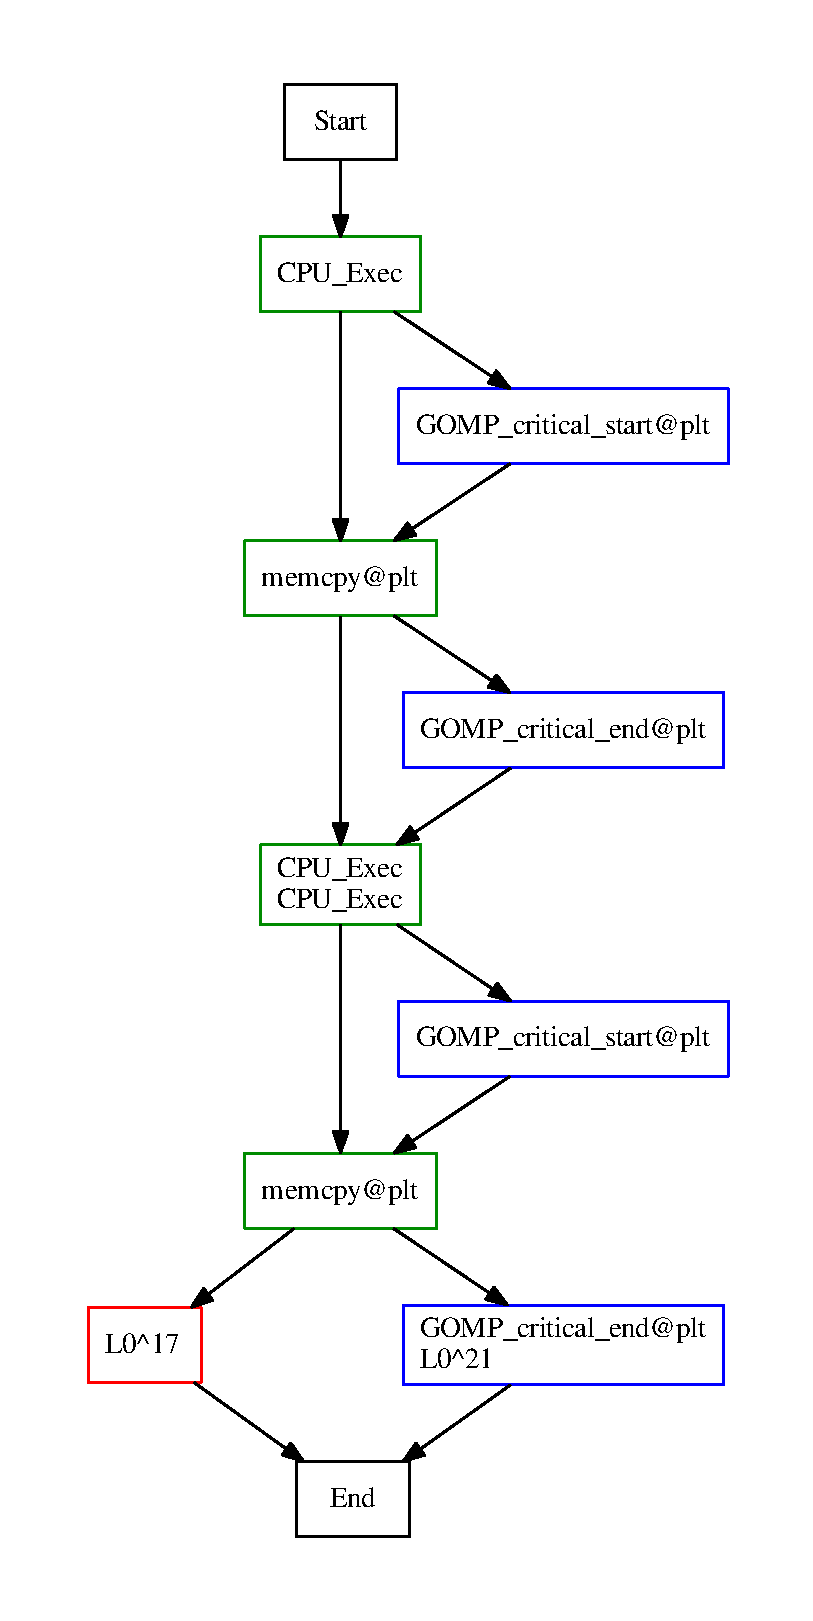
\includegraphics[width=0.3\textwidth]{figs/diffNLR/ompBug-6-4.pdf}
\caption{OpenMP Bug: diffNLR(6.4)}
\label{diffNLR-6-4}
\end{figure}

\subsection{MPI Bug: Deadlock Caused by Fault in Collectives}
By forcing only one of the processes (process 2) to invoke MPI\_Allreduce (line 24) with a wrong size, we have simulated a \textit{real deadlock}. 
%
Table~\ref{tab:ar1-ws-all-nn} shows that almost all processes are suspicious.
%
It turned out that ParLOT did not happen to capture function calls from all processes since the bug happens too early in the code. Thus except for process 1 and 4, all other traces are empty.
%
By looking at the diffNLR(1) (Figure~\ref{diffNLR-0}), we can see that both normal and the buggy trace of process $1$ are identical until an invocation of MPI\_Allreduce(). After that, normal trace hits the end of the program and terminates while the buggy process is waiting for the return from the actual point of fault (process 2) and never ends (i.e., deadlocks). 
%
diffNLRs of other processes look the same.
%


\begin{table}[]
\centering
\caption{Ranking table - MPI bug: wrong collective size in process 2}
\label{tab:ar1-ws-all-nn}
\scalebox{0.73}{
\begin{tabular}{|l|l|r|l|l|}
\hline
 Filter              & Attributes   &    B-score & Top Processes   & TOP Threads       \\
\hline
% 11.mem.mpicol.ompcrit.cust.0K10 & sing.log10   &      0.383 & 0 , 7 , 2 , 4 , 5 , 6 , & 1.1 , 1.3 , 1.4 , 3.1 , 3.2 , 3.4 , \\
% 11.mem.mpicol.ompcrit.cust.0K10 & sing.noFreq  &      0.383 & 0 , 7 , 2 , 4 , 5 , 6 , & 1.1 , 1.3 , 1.4 , 3.1 , 3.2 , 3.4 , \\
 11.mpicol.cust.0K10             & sing.log10   &      0.439 & 0 , 7 , 2 , 4 , 5 , 6  & 1.1 , 1.3 , 3.1 , 3.2 , 3.4        \\
 11.mpicol.cust.0K10             & sing.noFreq  &      0.439 & 0 , 7 , 2 , 4 , 5 , 6  & 1.1 , 1.3 , 3.1 , 3.2 , 3.4        \\
 11.mpi.cust.0K10                & doub.noFreq  &      0.457 & 0 , 7 , 2 , 4 , 5 , 6  & 1.4 , 3.3 , 3.4                    \\
 11.mpi.cust.0K10                & doub.actual  &      0.457 & 0 , 7 , 2 , 4 , 5 , 6  & 1.4 , 3.3 , 3.4                    \\
 11.mpiall.cust.0K10             & doub.noFreq  &      0.457 & 0 , 7 , 2 , 4 , 5 , 6  & 1.4 , 3.3 , 3.4                    \\
 11.mpiall.cust.0K10             & doub.actual  &      0.457 & 0 , 7 , 2 , 4 , 5 , 6  & 1.4 , 3.3 , 3.4                    \\
 11.mpicol.cust.0K10             & doub.noFreq  &      0.457 & 0 , 7 , 2 , 4 , 5 , 6  & 1.4 , 3.3 , 3.4                    \\
 11.mpicol.cust.0K10             & doub.actual  &      0.457 & 0 , 7 , 2 , 4 , 5 , 6  & 1.4 , 3.3 , 3.4                    \\
 11.mpi.cust.0K10                & sing.log10   &      0.465 & 0 , 7 , 2 , 4 , 5 , 6  & 1.1 , 1.3 , 3.1 , 3.2 , 3.4        \\
 11.mpi.cust.0K10                & sing.noFreq  &      0.465 & 0 , 7 , 2 , 4 , 5 , 6  & 1.1 , 1.3 , 3.1 , 3.2 , 3.4        \\
 11.mpiall.cust.0K10             & sing.log10   &      0.465 & 0 , 7 , 2 , 4 , 5 , 6  & 1.1 , 1.3 , 3.1 , 3.2 , 3.4        \\
 11.mpiall.cust.0K10             & sing.noFreq  &      0.465 & 0 , 7 , 2 , 4 , 5 , 6  & 1.1 , 1.3 , 3.1 , 3.2 , 3.4        \\
 11.mpi.cust.0K10                & doub.noFreq  &      0.543 & 0 , 7 , 2 , 4 , 5 , 6  & 1.4 , 3.3 , 3.4                    \\
 11.mpi.cust.0K10                & doub.actual  &      0.543 & 0 , 7 , 2 , 4 , 5 , 6  & 1.4 , 3.3 , 3.4                    \\
\hline
\end{tabular}}
\end{table}


\begin{figure}[]
\centering
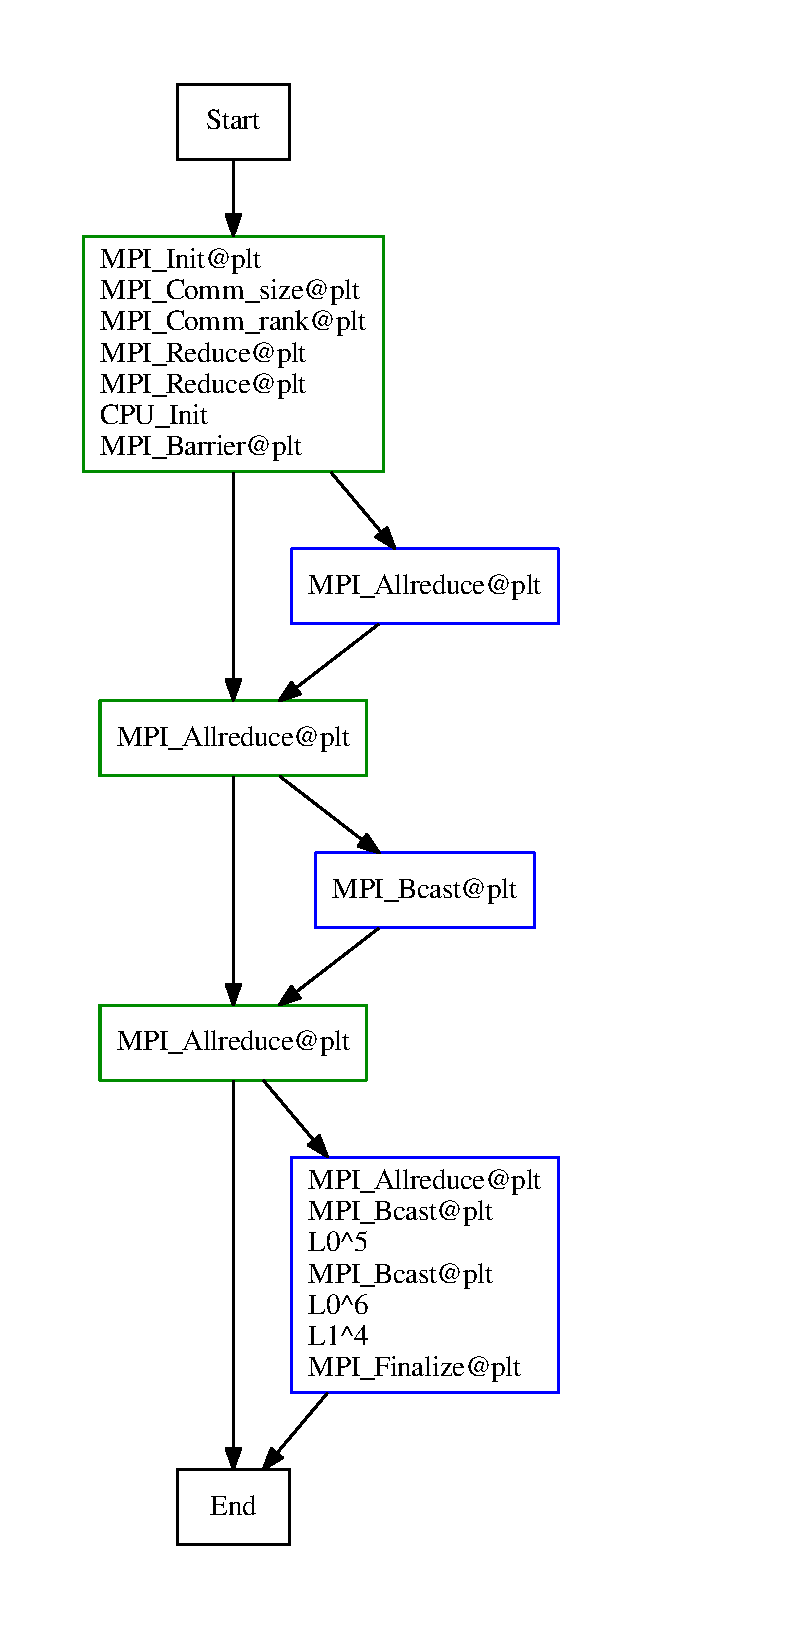
\includegraphics[width=0.3\textwidth]{figs/diffNLR/mpiBug-all-nn.pdf}
\caption{diffNLR(0)}
\label{diffNLR-0}
\end{figure}
%



\subsection{MPI Bug: Wrong Collective Operation}
By changing the operation MPI\_MIN to MPI\_MAX in the input arguments of MPI\_Allreduce(), we have changed the semantics of ILCS. 
%
The execution of this variation terminated well, but the results might be corrupted.
%

The MPI\_Allreduce() in line 24 of Listing~\ref{lst:ilcs} broadcasts the best-calculated answer among all processes.
%
However, by the change that we made to ILCS, now the ``worst'' answer is getting stored.
%
We injected the bug only to process 0.
%
Among all suggested suspicious processes (Table~\ref{tab:ar1-wo-0-nn}), only process 5 (bold numbers) are making sense since their filters are more relevant to the aspect that we are interested (MPI-level activities) to study deeper.
%
Our observation from diffNLR(5) (Figure~\ref{diffNLR-5}) is that process 5, in comparison with its corresponding normal process, involves more in updating and broadcasting the champion among all traces.
%
Similar to the deadlock bug, this is another instance of  ``bug manifestation'' detection by DiffTrace.

\begin{table}[]
\centering
\caption{Ranking Table - MPI-Bug: Wrong Collective Operation ,Injected to Process 0}
\label{tab:ar1-wo-0-nn}
\scalebox{0.72}{
\begin{tabular}{|l|l|r|l|l|}
\hline
 Filter              & Attributes   &    B-score & Top Procs ($JSM_D$)   & TOP Threads($JSM_D$)             \\
\hline
 01.plt.cust.0K10    & doub.log10   &      0.271 & 2 ,                & 6.2 , 7.3 , 2.2 , 5.2 , 5.3 , \\
 11.plt.cust.0K10    & doub.log10   &      0.271 & 2 ,                & 6.2 , 7.3 , 2.2 , 5.2 , 5.3 , \\
 01.plt.cust.0K10    & sing.actual  &      0.276 & 1 ,                & 3.1 , 1.4 , 6.4 , 3.4 ,       \\
 11.plt.cust.0K10    & sing.actual  &      0.276 & 1 ,                & 3.1 , 1.4 , 6.4 , 3.4 ,       \\
 01.plt.cust.0K10    & doub.noFreq  &      0.285 & 2 ,                & 6.2 , 7.3 , 2.2 , 5.2 , 5.3 , \\
 11.plt.cust.0K10    & doub.noFreq  &      0.285 & 2 ,                & 6.2 , 7.3 , 2.2 , 5.2 , 5.3 , \\
 01.plt.cust.0K10    & sing.log10   &      0.292 & 1 , 4 , 5 , 6 ,    & 3.1 , 4.3 ,                   \\
 11.plt.cust.0K10    & sing.log10   &      0.292 & 1 , 4 , 5 , 6 ,    & 3.1 , 4.3 ,                   \\
 01.\textbf{mpicol}.cust.0K10 & sing.actual  &      0.312 & \textbf{5} ,                & 3.2 , 6.4 , 5.4 , 4.2 ,       \\
 11.\textbf{mpicol}.cust.0K10 & sing.actual  &      0.312 & \textbf{5} ,                & 3.2 , 6.4 , 5.4 , 4.2 ,       \\
 11.\textbf{mpi}.cust.0K10    & sing.actual  &      0.331 & \textbf{5} ,                & 3.2 , 6.4 , 5.4 , 4.2 ,       \\
 11.\textbf{mpiall}.cust.0K10 & sing.actual  &      0.331 & \textbf{5} ,                & 3.2 , 6.4 , 5.4 , 4.2 ,       \\
 01.\textbf{mpiall}.cust.0K10 & sing.actual  &      0.331 & \textbf{5} ,                & 3.2 , 6.4 , 5.4 , 4.2 ,       \\
 01.\textbf{mpi}.cust.0K10    & sing.actual  &      0.331 & \textbf{5} ,                & 3.2 , 6.4 , 5.4 , 4.2 ,       \\
 11.\textbf{mpi}.cust.0K10    & sing.actual  &      0.371 & \textbf{5} ,                & 3.2 , 6.4 , 5.4 , 4.2 ,       \\
 11.\textbf{mpiall}.cust.0K10 & sing.actual  &      0.371 & \textbf{5} ,                & 3.2 , 6.4 , 5.4 , 4.2 ,       \\
\hline
\end{tabular}}
\end{table}


\begin{figure}[]
\centering
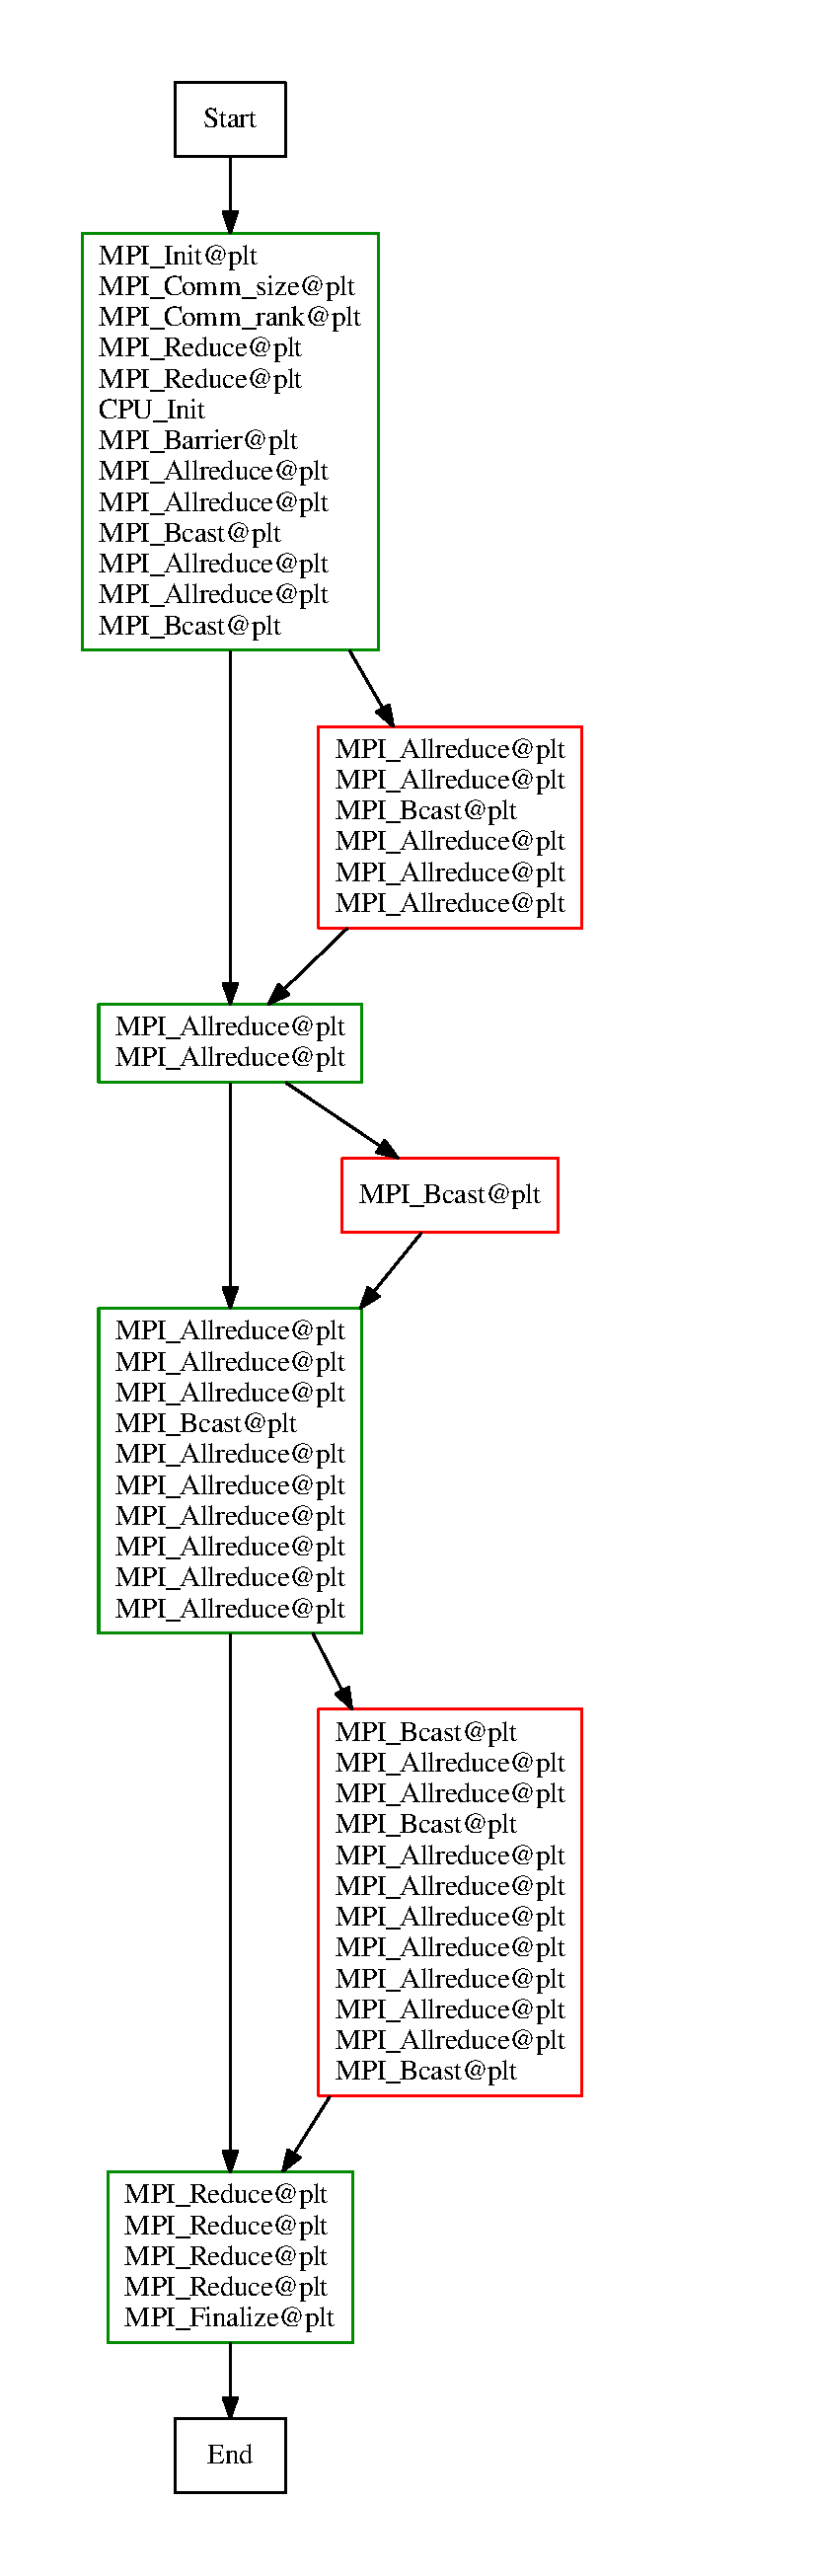
\includegraphics[width=0.3\textwidth]{figs/diffNLR/mpiBug2-0-nn.pdf}
\caption{diffNLR(5)}
\label{diffNLR-5}
\end{figure}


